\chapter{Lecture 2: Tolerant Retrieval}
\begin{multicols*}{2}

\noindent Parsing document: format and language of documents, granularity of documents \\

\noindent Case folding: just lowercase everything

\section{Tokenisation}
\noindent Issues: handling apostrophe, hyphenation, names of places / cities, date in various formats, telephone numbers \\

\noindent Language issues: different languages, languages without spaces between words, multiple formats in Japanese language, language written from right to left

\section{Stopwords}
\noindent Stopwords are common words in a language. Stopwords are important for phrase queries, song titles and relational queries (e.g. flights to London)

\section{Normalisation}
\noindent We need to normalise words in indexes and queries into the same form. For example, deleting periods (U.S.A $\rightarrow$ USA), hyphens, accents, umlauts, and date formats.

\section{Thesauri and Soundex}
\noindent To handle synonyms and different spellings, we can manually construct equivalence classes. For example, when the query is ``car'', we also do a query expansion to search for ``automobile''. \\

\noindent Spelling mistakes can be handled by Soundex, which forms equivalence classes of words based on phonetic heuristics.

\section{Lemmatisation}
Reduce variant forms to base form. For example:
\begin{itemize}
    \item car cars car’s cars’ $\rightarrow$ car
    \item am are is $\rightarrow$ be
\end{itemize}

\section{Stemming}
\noindent Reduce terms to their “roots”, by crude chopping, while preserves part-of-speech (POS) tags. For example:
\begin{itemize}
    \item automates automatic automation $\rightarrow$ automat
    \item democrats $\rightarrow$ democrat (noun)
    \item democratised $\rightarrow$ democratize (verb)
\end{itemize}
\noindent Lemmatisation reduce variant in noun or verb, but may lead to misunderstanding. 

\section{Wild-card Queries}
\noindent We want to query \verb|mon*|, means any words that start with \verb|mon|. We can build a binary tree lexicon and retrieve all words in range $\verb|mon|\le w < \verb|moo|$. \\

\noindent There are three solution to handle wild-card queries in the middle of query term (\verb|co*tion|). The first solution is by looking up words start with the prefix (\verb|co*|) and find all terms end with the suffix (\verb|tion|). The second solution is by looking up the prefix and suffix in two different binary tree and intersect the two term sets. The last solution is permuterm index. 

\subsection{Permuterm Index}
\noindent Transform wild-card queries so that the * occurs at the end. For example, for the term hello index under \verb|hello$ ello$h llo$he lo$hel o$hell|. \\

\noindent For query processing, we rotate the query wild-card to the right and look up in respective binary tree as before. 

\section{Spell Correction}
\subsection{Edit / Levenshtein Distance}
\noindent Given two string, find the minimum number of operations to convert to one to the other. The operations are:
\begin{itemize}
    \item insert, delete, replace (distance = 1)
    \item transposition (distance = 2)
\end{itemize}

\noindent Example of Levenshtein Distance:
\begin{center}
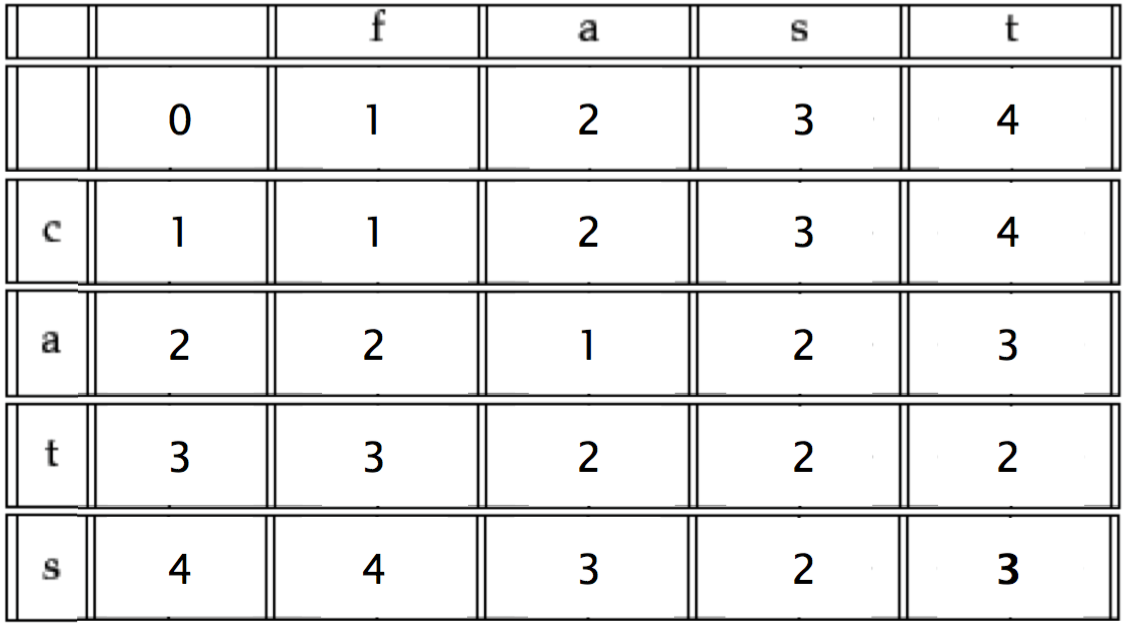
\includegraphics[width=8cm]{levenshtein}
\end{center}

\noindent However, there are too many dictionary term to compare. We can cut the candidate terms using n-gram overlap.

\subsection{N-gram Overlap and Jaccard Coefficient}
\noindent N-gram overlap can be used by itself for spell correction. Example of n-gram overlap:
\begin{itemize}
    \item november: \verb|nov ove vem emb mbe ber|
    \item december: \verb|dec ece cem emb mbe ber|
    \item So \verb|ebb mbe ber| are overlap
\end{itemize}

\noindent We then apply Jaccard coefficient:
$$J=\frac{X\cap Y}{X\cup Y}$$

\subsection{Isolated Word Correction}
\noindent Assumption: there is a lexicon from which the correct spellings come.  \\

\noindent Given a lexicon and a character sequence Q, return the words in the lexicon closest to Q. The closeness is based on either edit distance or n-gram overlap. 

\subsection{Context-sensitive Correction}

\noindent Need surrounding context to recommend a statistically more plausible alternative. \\

\noindent Solution 1: Retrieve dictionary term close to each query term, then try all possible resulting phrase with one word fixed at a time. Finally, suggest the alternative that has lots of hits
\begin{itemize}
    \item flew from heathrow
    \item fled form heathrow
    \item flea form heathrow
\end{itemize}

\noindent Solution 2: generalisation. For example, \verb|fly_from|, \verb|fly_to|,\verb|fly_through|, \verb|fly_away|. \\

\noindent Solution 3: Break phrase query into biwords, look for biwords that need only one term corrected, and rank them. 

\end{multicols*}
